%!TEX root = HICSS51.tex
In this section, the structure of the bi-level optimization problem is described. The general formulation of a bilevel optimization is given below:

\begin{align}
\begin{aligned}
&\argminC_{x\in X, y\in Y}F\left(x,y\right) \\
\text{st:   }  & G_i\left(x,y\right)\leq 0, \text{for   }  i \in \{1,2,...,I\}\label{prime}\\
& H_k\left(x,y\right) = 0, \text{for   }  k \in \{1,2,...,K\}\\
& y\in \argminB_{y\in Y} \{f(x,y): g_j(x,y)\leq 0, \text{for   }  j \in \{1,2,...,J\}, \\ 
                                                   &h_m(x,y) = 0, \text{for   }  m \in \{1,2,...,M\}  \}
\end{aligned}
\end{align}


In the above formulation, $x,F(x,y),(G_i, H_k)$ are the optimization variables, objective function and constraints of the upper level problem. Whereas, $y,f(x,y),(g_i,h_m)$ are the optimization variables, objective function and constraints of the lower level problem. According to this formulation, the bilevel formulation of the TS and DS co-optimization is given in the following sections. 

\subsection{Upper Level Problem: TS Unit Commitment Problem}

The upper level transmission day-ahead unit commitment problem seeks to compute the optimal operation schedule including the generator commitment status $w_{g,t}$, generation output $p_{g,t}$, upward and downward generator's reserve $R^{up}_{g,t}$, $R^{dn}_{g,t}$, DS DR price $P^{dr}_{g,t}$, and the DS energy import $c^{im}_{t}$ to minimize the total TS operation cost. The optimization variables are denoted by the vector $x_t$, and include:
\begin{align*}
x_t=[&w_{g,t}, p_{g,t}, r_{g,t}^{up}, r_{g,t}^{dn}, p^{dr}_{t}, c^{im}_{t}]
\end{align*}
The objective of the upper level optimization problem is to minimize the TS operation cost including the generator commitment cost, generation cost, reserve cost,  the DISCO DR cost, and negative DISCO energy import cost. \\
\textbf{\emph{Objective function:} }
\begin{equation*}
\begin{array}{lcl}
F(\{x_t\}^{T}_{t=1}) &=& \sum_{t=1}^{T}\sum_{g=1}^{G}(C^c_{g,t} w_{g,t}+C_{g,t} p_{g,t}\\
&+&C^r_{g}(r_{g,t}^{up}+r_{g,t}^{dn})+p^{dr}_{t}(dr_{t}^{up}+dr_{t}^{dn})\\
&-&p^{im}_{t}c^{im}_{t})
\end{array}
\label{eqn:obj}
\end{equation*}

The constraints of the TS are listed below. \\
\textbf{\emph{Power flow constraints:} }
\begin{align}
&-Line\leq GSF*p^{inj}_{t}\leq Line, t\in{1,...,T}\label{eqn:1}\\
&-Line\leq GSF*p^{inj*}_{t}\leq Line, t\in{1,...,T}\label{eqn:2}
\end{align}

$p^{inj}_{t}$ is the DC net power injection vector (ie: generation + wind - demand) for all the buses in each hour. $p^{inj*}_{t}$ incorporates the wind forecast error, generator reserve and MG DR on top of $p^{inj}_{t}$. Eqn (\ref{eqn:1}),(\ref{eqn:2})  bound the transmission line flows within the flow limits. 
 
\textbf{\emph{Generator constraints:} }
\begin{align}
& \underline{P}_g\leq p_{g,t}\leq  \overline{P}_g,  t\in{1,...,T}\label{eqn:dtpg}\\
& (p_{g,t} +r_{g,t}^{up})  - (p_{g,t-1}-  r_{g,t-1}^{dn}) \leq \overline{R}_g ,  t\in{2,...,T}\label{eq: sec3} \\
&  \underline{R}_{g} \leq (p_{g,t} -  r_{g,t}^{dn})  - (p_{g,t-1}+ r_{g,t-1}^{up}) , t\in{2,...,T}\label{eq: sec4} 
\end{align}

Eqn (\ref{eqn:dtpg}) bounds the generator generation within its capacities. Eqn (\ref{eq: sec3}),(\ref{eq: sec4}) satisfy the generator ramping capability. 

\textbf{\emph{Power balance constraint:} }
\begin{align}
\sum_{g=1}^{G} p_{g,t} + \mathbf{1}_{1\times N_b}*L_{t} + W^f = p^{im}_t, ,  t\in{1,...,T}\label{eq: sec5} 
\end{align}
where $\mathbf{1}_{1\times N_b}$ is a vector of length $N_b$ filled with 1's. The dot product $\mathbf{1}_{1\times N_b}*L_{t}$ gives the total load in the system. Eqn (\ref{eq: sec5}) balances the system power supply and demand. 

\textbf{\emph{Reserve constraints:} }

\begin{align}
W^{up}_t \leq dr^{up}_t + \sum_{g=1}^{G} r_{g,t}^{dn}, t\in{1,...,T} \label{xx} \\
W^{dn}_t \leq dr^{dn}_t + \sum_{g=1}^{G} r_{g,t}^{up}, t\in{1,...,T} \label{eq: sec7} 
\end{align}

Eqn (\ref{xx}), (\ref{eq: sec7}) ensure enough generator reserve and MG DR to compensate the possible wind forecast deviation. 

Finally, the TS unit commitment problem is formulated as: 

\begin{align}
\text{min}_{\{x_t\}^{T}_{t=1}} & F\left(\{x_t\}^{T}_{t=1}\right)\nonumber
\end{align}

\subsection{Lower Level Problem: DS Operation Optimization}
The DS considered in this work has a radial network as shown in Fig.~\ref{pf}. There are n buses in the network indexed by $i = 0,1,..., n.$ A simplified version of power flow that only considers active power according to ~\cite{dpf} is considered in this work. The power flow equation at each node $i$ could be expressed as

\begin{align}
& P_{i+1} = P_i - p_{i+1}\nonumber \\
& p_{i} =  L^i_{} + l^d_{} \nonumber 
\end{align}

$p_{i}$ is the net load at bus i. 

\begin{figure}
\centering
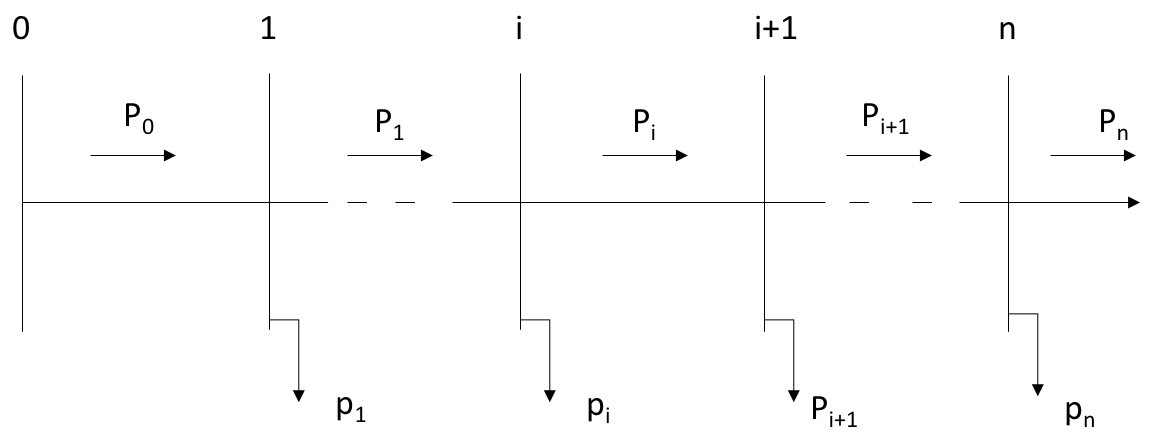
\includegraphics[scale=0.2]{pfs.png}
\caption{Diagram of a radial distribution network}
\label{pf}
\end{figure}

The DS could only import energy from the transmission system. The load in the DS is served by the DS DG as well as the TS energy import.

The goal of the DS optimization problem is to compute the energy import $p^{im}_{t}$ schedule, dispatchable load profile $l^d_{t}$, the upward/downward DR $dr_{t}^{up}$, $dr_{t}^{dn}$ provided by the dispachable load. The lower level optimization variables are denoted by the vector $y_t$, and include:
\begin{align*}
y_t=[&p^{im}_{t}, dr_{i,t}^{up},dr_{i,t}^{dn},l^d_{i,t}]
\end{align*} 

The objective of the DS optimization is to minimize the DS operation cost including its DG cost,  energy import cost from the TS, and DR cost and maximize its DL utility and DR revenue.

\textbf{\emph{Objective function:}}
\begin{align*}
f(\{y_t\}^{T}_{t=1}) =& \sum_{t=1}^{T}\sum_{i=1}^{N^d_b}(C^{d1}_i p^d_{i,t} +C^{d2}_g p^d_{i,t}  p^d_{i,t} +p^{im}_{t}c^{im}_{t}\\
+ &C^{dr1} (dr^{up}_{i,t} + dr^{dn}_{i,t} ) \\
+ &C^{dr2} (dr^{up}_{i,t}dr^{up}_{i,t} + dr^{dn}_{i,t}dr^{dn}_{i,t}  ) \\
+ &C^{d}(\overline{P}^d_{i}-p^d_{i,t})(\overline{P}^d_{i}-p^d_{i,t})\\
- &p^{dr}_{t}(dr_{i,t}^{up}+dr_{i,t}^{dn}))
\end{align*}

The constraints for the DS are given below. The $\lambda$ and $\mu$ variables next to the constraints are the dual variables associated with the corresponding inequality and equality constraints.

%\textbf{\emph{DG constraints:} }
%\begin{align}
%&\underline P^d_{i}\leq p^d_{i}\leq  \overline P^d_{i}\label{genlim}, \lambda_{1,i,t},\lambda_{2,i,t},t\in{1,...,T} ,i\in{1,...,N_b^d} 
%\end{align}
%Eq (\ref{genlim}) limits the generator's output within the upper and lower bound.\\

\textbf{\emph{Power flow constraints:} }
\begin{align}
& P_{i+1,t} = P_{i,t} - (L^{ie}_{i,t} + l^d_{i,t} - p^d_{i,t}) \nonumber\\
& t\in{1,...,T} ,\mu_{1,i,t},i\in{1,...,N_b^d}  \label{pfc}\\
&  \underline P_{i} \leq P_{i,t} \leq  \overline P_{i}, t\in{1,...,T}, \lambda_{3,i,t},\lambda_{4,i,t}, i\in{1,...,N_b^d}\label{pfcs}
\end{align}
Eq (\ref{pfc}) regulates the power flow between nodes in the distribution system. Eq (\ref{pfcs}) bounds the power flow within the line limits in the distribution system. Note that $P_{1,t}$ is the DS energy import $p^{im}_t$. \\

\textbf{\emph{Dispatchable load constraint:} }
\begin{align}
&\underline{L}^d_{i}\leq l^d_{i}\leq \overline{L}^d_{i,t}\label{dl}, \lambda_{5,i,t},\lambda_{6,i,t},t\in{1,...,T},i\in{1,...,N_b^d} 
\end{align} 
Eq (\ref{dl}) constrains the dispatchable loads within predefined bounds. 

\textbf{\emph{DR constraints:} }
\begin{align}
&0\leq dr_{i,t}^{up}\leq S^(dr)*l^{i,d}_t, \lambda_{7,i,t},\lambda_{8,i,t},t\in{1,...,T}, i\in{1,...,N_b^d}  \label{dlu1}\\
&0\leq dr_{i,t}^{dn}\leq S^(dr)*l^{i,d}_t, \lambda_{9,i,t},\lambda_{10,i,t},t\in{1,...,T}, i\in{1,...,N_b^d}  \label{dlu2}
\end{align} 
The amount of DR is set to be within a certain percentage defined by the DR scale factor $S^(dr)$ of the DL, which is reflected in Eq (\ref{dlu1}), (\ref{dlu2}).

%\textbf{\emph{Import and Export constraints:} }
%\begin{align}
%& 0 \leq  p^{im}_t, \lambda_{9,t}, t\in{1,...,T} \label{dlu3}
%\end{align}
%The DG import power is defined to be non-negative as shown in Eqn (\ref{dlu3}).
%
%\textbf{\emph{Power balance constraint:} }
%\begin{align}
%&p^d_{t} -L^i_{t}-l^d_{t} = -p^{im}_{t}, \mu_{2,t}, t\in{1,...,T}\label{6}
%\end{align}
%Eq (\ref{6}) ensures the power balance within the MG system.\\

Finally, the MG optimal dispatch can be formulated as: 
\begin{subequations}
\begin{align}
\text{min}_{\{y_t\}^{T}_{t=1}} & f\left(\{y_t\}^{T}_{t=1}\right)\nonumber\\
\text{s.t.  }  & (10) - (15)\nonumber
\end{align}
\end{subequations}

\subsection{Reformulation to a Single Level Problem}
If the lower level problem is convex and satisfies certain regularity conditions \cite{convex}, it can be replaced by its Karush-Kuhn-Tucker(KKT) conditions \cite{bilevel1}, the formulation in (\ref{prime}) becomes a single -level problem reformulation as follows:


\begin{align}
&\argminC_{x\in X, y\in Y}F\left(x,y\right)\nonumber\\
\text{st:  } & G_i\left(x,y\right)\leq 0, \text{for   }  i \in \{1,2,...,I\}\nonumber\\
& H_k\left(x,y\right)= 0, \text{for   }  k \in \{1,2,...,K\}\nonumber\\
&g_i\left(x,y\right)\leq 0, \text{for   }  j \in \{1,2,...,J\}\nonumber\\
&h_m\left(x,y\right)\leq 0, \text{for   }  m \in \{1,2,...,M\}\nonumber\\
&\text{dual feasibility: }\lambda_i\geq 0, \text{for   }  i \in \{1,2,...,I\}\nonumber\\
&\text{complementary slackness: }\nonumber \\
&\lambda_i*g_i\left(x,y\right)= 0, \text{for   }  i \in \{1,2,...,I\}\nonumber\\ 
&\text{stationarity: }\nabla \textit{L}(x,y,\lambda,\mu)=0\nonumber\\ 
& where:\nonumber\\ 
 &  \textit{L}(x,y,\lambda)=f(x,y)+\sum_{i=1}^{J}\lambda _ig_i(x,y)+\sum_{m=1}^{M}\mu _mh_m(x,y)\nonumber
\end{align}


The lower level problem in this study is a convex optimization problem and satisfies Slater's condition, which is one of the sufficient conditions for strong duality theorem \cite{convex}. Therefore, the lower level problem could be replaced by its KKT conditions. The KKT conditions are given below:\\

\textbf{\emph{Stationarity}}: \\
For stationarity, the derivative of the lagrangian function  $\textit{L}(x,y,\lambda)$ is taken with respect to each optimization variable. For example, eq(\ref{lam1}) is the derivative of the lagrangian function with respect to $p^d_{i,t}$.
\begin{align}
& 2*C^{d2}_i*p^d_{i,t} + C^{d1}_i + \lambda_{2,i,t}-\lambda_{1,i,t}+\mu_{1,i,t} =0 \nonumber\\ 
& t\in{1,...,T},i \in \{1,...,N^d_b\} \label{lam1}\\
& 2*C^{dr2}_i*dr^{up}_{i,t} + C^{dr1}_i - p ^{dr}_t + \lambda_{8,i,t}-\lambda_{7,i,t} =0 \nonumber\\ 
& t\in{1,...,T},i \in \{1,...,N^d_b\}  \\
& 2*C^{dr2}_i*dr^{up}_{i,t} + C^{dr1}_i - p ^{dr}_t + \lambda_{8,i,t}-\lambda_{7,i,t} =0 \nonumber\\ 
& t\in{1,...,T},i \in \{1,...,N^d_b\} \\
& p^{im}_t -\mu_{1,1,t}+ \lambda_{4,1,t}-\lambda_{3,1,t} =0, t\in{1,...,T}, i=1 \\
& \mu_{1,i-1,t} -\mu_{1,i,t}+ \lambda_{4,i,t}-\lambda_{3,i,t} =0,  \nonumber\\ 
& t\in{1,...,T},i \in \{2,...,N^d_b\} \\
%& \mu_{1,i-1,t} -\mu_{1,i,t}+ \lambda_{4,i,t}-\lambda_{3,i,t} =0, t\in{1,...,T} \\
& 2*C^{d}*l^d_{1,t} + C^{d}*\overline{L}^d_{i,t} + \lambda_{6,1,t}-\lambda_{5,1,t}\nonumber\\
&-\lambda_{8,1,t}-\lambda_{10,1,t} =0 , t\in{1,...,T}, i = 1  \label{lam1}\\
& 2*C^{d}*l^d_{i,t} + C^{d}*\overline{L}^d_{i,t} + \lambda_{6,i,t}-\lambda_{5,i,t}\nonumber\\
& -\lambda_{8,i,t}-\lambda_{10,i,t}+\mu_{1,i,t}=0 , t\in{1,...,T}, i\in{2,...,N^d_b}  \label{lam1}
\end{align}

 \textbf{\emph{Dual feasibility}}: \\
For dual feasibility, all dual variables need to be non-negative.
\begin{align}
\lambda_{1,t} ... \lambda_{10,t} , t\in{1,...,T} \geq 0 
\end{align}
\textbf{\emph{Complementary slackness}}: \\
For complementary slackness, the product of the dual variables and their corresponding inequalities need to be zero.
\begin{align}
& \lambda_{1,i,t}*(p^d_{i,t}-\underline P^d_i) = 0, t\in{1,...,T}, i\in{1,...,N^d_b}  \\
& \lambda_{2,i,t} *(p^d_{i,t}-\overline P^d_i) = 0 , t\in{1,...,T}, i\in{1,...,N^d_b}  \\
& \lambda_{3,i,t}*(P_{i,t}-\overline P_i) = 0 , t\in{1,...,T}, i\in{1,...,N^d_b}  \\
& \lambda_{4,i,t}*(P_{i,t}-\underline P_i) = 0 , t\in{1,...,T}, i\in{1,...,N^d_b}  \\
& \lambda_{5,i,t}*(l^d_{i,t}-\overline L^d_{t}) = 0 , t\in{1,...,T} , i\in{1,...,N^d_b} \\
& \lambda_{6,i,t}*(l^d_{i,t}-\underline L^d_t) = 0 , t\in{1,...,T}, i\in{1,...,N^d_b}  \\
& \lambda_{7,i,t}*dr_{i,t}^{up} = 0 , t\in{1,...,T} , i\in{1,...,N^d_b} \\
& \lambda_{8,i,t}*(dr_{i,t}^{up}-0.2*l^d_{i,t}) = 0 , t\in{1,...,T} , i\in{1,...,N^d_b} \\
& \lambda_{9,i,t}*dr_{i,t}^{dn} = 0, t\in{1,...,T} , i\in{1,...,N^d_b}  \\
& \lambda_{10,i,t}*(dr_{i,t}^{dn}-0.2*l^d_{i,t}) = 0 , t\in{1,...,T} , i\in{1,...,N^d_b} 
\end{align}

This reformulation is not easy to solve mainly due to the non-convexity in the complementary slackness and bilinear terms in the objective function. The big-M reformulation is used to transform the complementary conditions to mixed integer constraints. The technical details of the Big-M method is given in the appendix. 

According to strong duality theorem, the optimal objective function value of the lower level optimization dual problem equals the optimal objective function value of the lower level optimization primal problem.  As a result, the bilinear terms $-p^{im}_{t}c^{im}_{t}+p^{dr}_{t}(dr_{t}^{up}+dr_{t}^{dn})$ in the lower level objective function, which also appear in the upper level objective function, could be expressed as linear terms using the objective function of the dual problem. The lower level dual problem objective function is as follow:\\
\begin{equation*}
\begin{array}{lcl}
D(\{\lambda_t,\mu_t\}^{T}_{t=1}) &=& \sum_{t=1}^{T}\sum_{i=1}^{N^d_b}(-C^{d2}p^{d}_{i,t}p^{d}_{i,t} - C^{ld}l^{d}_{i,t}l^{d}_{i,t} \\
&-& l^{d}_{i,t}\mu_{i,t} + \lambda_{3,i,t} \underline{P}_{i,t} -\lambda_{4,i,t} \overline{P}_{i,t} \\
&+&\lambda_{5,i,t} \overline{L}^{d}_{i,t} -\lambda_{6,i,t} \underline{L}^{d}_{i,t}\\
&+&\lambda_{1,i,t} \overline{P}^{d}_{i} -\lambda_{2,i,t} \underline{P}^{d}_{i})
\end{array}
\label{eqn:obj}
\end{equation*}

The bilinear terms $-p^{im}_{t}c^{im}_{t}+p^{dr}_{t}(dr_{t}^{up}+dr_{t}^{dn})$ in the upper level objective function are represented as:
\begin{align*}
y = & \sum_{t=1}^{T}\sum_{i=1}^{N^d_b}(C^{d1}_i p^d_{i,t} +C^{d2}_g p^d_{i,t}  p^d_{i,t} \\
+ &C^{dr1} (dr^{up}_{i,t} + dr^{dn}_{i,t} ) \\
+ &C^{dr2} (dr^{up}_{i,t}dr^{up}_{i,t} + dr^{dn}_{i,t}dr^{dn}_{i,t}  ) \\
+ &C^{d}(\overline{P}^d_{i}-p^d_{i,t})(\overline{P}^d_{i}-p^d_{i,t})) - D(\{\lambda_{i,t},\mu_{i,t}\}^{T,N^d_b}_{t=1,i=1}) 
\end{align*}

%\begin{align*}
%\sum_{t=1}^{T}(C^{m1}_g p^m_{g,t} +C^{m2}_g p^m_{g,t}  p^m_{g,t} +C^bb_t + C^{dr1} dr^{up}_{g,t} + dr^{dn}_{g,t}  +\\
%+C^{dr2} (dr^{up}_{g,t}dr^{up}_{g,t} + dr^{dn}_{g,t}dr^{dn}_{g,t}  ) - C^d_{t}l^d_{t}) - D(\{\lambda_{i,t},\mu_{i,t}\}^{T,N^d_b}_{t=1,i=1}) 
%\end{align*}

The reformulated upper level objective function is as follow:\\
\begin{equation*}
\begin{array}{lcl}
F\left(\{x_t,y_t, \lambda_{t,i}, \mu_{t,i}\}^{T,N^d_b}_{t=1,i=1}\right) &=& \sum_{t=1}^{T}\sum_{g=1}^{G}(C^c_{g,t} w_{g,t}+C_{g,t} p_{g,t} \\
&+&C^r_{g}(r_{g,t}^{up}+r_{g,t}^{dn}) - y
\end{array}
\label{eqn:obj}
\end{equation*}

The reformulated single level problem has the following format:\\
\begin{subequations}
\begin{align}
\text{min}_{\{x_t,y_t, \lambda_t, \mu_t\}^{T}_{t=1}} & F\left(\{x_t,y_t, \lambda_t, \mu_t\}^{T}_{t=1}\right)\nonumber\\
\text{st:   } & (2)-(34)\nonumber
\end{align}
\end{subequations}

With the big-M reformulation, a set of binary variables and additional constants are introduced. The bilevel problem becomes a single level mixed integer linear problem and could thus be solved with a wide range of commercial solvers such as Cplex and Gurobi. 

